\section{Performance Evaluation}
\label{sec:jnif-evaluation}

We evaluated the performance of a JNIF-based dynamic instrumentation approach 
versus an approach using an ASM-based instrumentation server.

\subsection*{Measurement Contexts}

%\todo{Stecklov?}
%\todo{Yudi's machine?}
%\todo{Luis' Mac?}
We ran our experiments on three different machines:
(1) A machine with two Intel Xeon E5-2620 2~GHz CPUs, 
each with 6 cores and 2 threads per core, 
and 8~GB RAM,
running Debian Linux x86 64 3.10.11-1.
(2) A Dell PowerEdge M620, 2 NUMA node with 64 GB of RAM, 
Intel Xeon E5-2680 2.7~GHz CPU
with 8 cores, 
CPU frequency scaling and Turbo Mode disabled,
running Ubuntu Linux x86 64 3.8.0-38.
For consistent memory access speed, 
we bound our program to a specific NUMA node using \texttt{numactl}.
(3) A MacBook Pro with an Intel Core i7 2.7~GHz CPU 
with 4 cores and 16~GB
running Mac OS X 10.8.2.

%
%For consistent memory access speed, you should add the following before your command,
%which will bind your program in the same NUMA node.
%numactl --cpubind=0 --membind=0
%or
%numactl --cpubind=1 --membind=1




\subsection*{Benchmarks}

We used the Dacapo benchmarks, 
except for tradebeans and tradesoap,
which suffer from a well known issue\footnote{\url{http://sourceforge.net/p/dacapobench/bugs/70/}}.
We also include the Scala benchmarks (except for the subset identical to Dacapo).


%\subsection{Metrics}
%We compare several aspects between the instrumentation made by JNIF and ASM.
%These aspects include time and memory.



\subsection*{Subjects}
We compare JNIF to ASM for the purpose of performing dynamic instrumentation.
For JNIF we built a JVMTI agent that directly includes JNIF to instrument loaded classes.
For ASM, we use a JVMTI agent that forwards loaded classes to an instrumentation server
that uses ASM's streaming API (which is faster than ASM's tree API).


\subsection*{Results}

Figure~\ref{fig:instr-time} shows the results of our performance evaluation
in terms of time spent instrumenting classes.
The figure shows the results from our first machine.
The other machines produced results similar to Figure~\ref{fig:instr-time}, 
and we omit them for space reasons.
The figure shows box plots summarizing five measurement runs.
It shows one box for JNIF and two boxes for ASM.
The ``ASM Server'' box represents the time as measured on the instrumentation server.
This is equivalent to the time a static instrumentation tool would take.
It excludes the time spent in the JVMTI agent and the time for the IPC between the agent and the server.
The ``ASM Server on Client'' box represents the total time needed for instrumentation, 
as measured in the JVMTI agent,
and thus includes the IPC and JVMTI agent time.

Each chart in the figure consists of five groups of boxes:
``Empty'' is the time when using a JVMTI agent that does not process bytecodes at all.
``Identity'' is for an agent that simply decodes and encodes each class, without any instrumentation, and without recomputing stack maps.
``ComputeFrames'' also includes recomputing stack maps.
``Allocations'' represents a useful dynamic analysis that captures all allocations.
``Nop Padding'' is a different dynamic analysis that injects NOPs after each bytecode instruction. 

The figure shows that frame computation adds significant overhead, on ASM as well as JNIF.
Moreover, it shows that except for dacapo-eclipse, dacapo-jython, and scala-scalatest,
JNIF is faster even than just the ASM Server time.

% \ignore{
% \begin{figure*}[htb]
% \centering
% \vspace{-1cm}
% \includegraphics[width=\textwidth]{../eval-dacapo-chart-instr}

% \vspace{-5mm}
% \includegraphics[width=\textwidth]{../eval-scala-chart-instr}

% \vspace{-5mm}
% \caption{Instrumentation time on DaCapo and Scala benchmarks}
% \label{fig:instr-time}
% \end{figure*}
% }

\begin{figure*}[htb]
\centering
\vspace{-1cm}
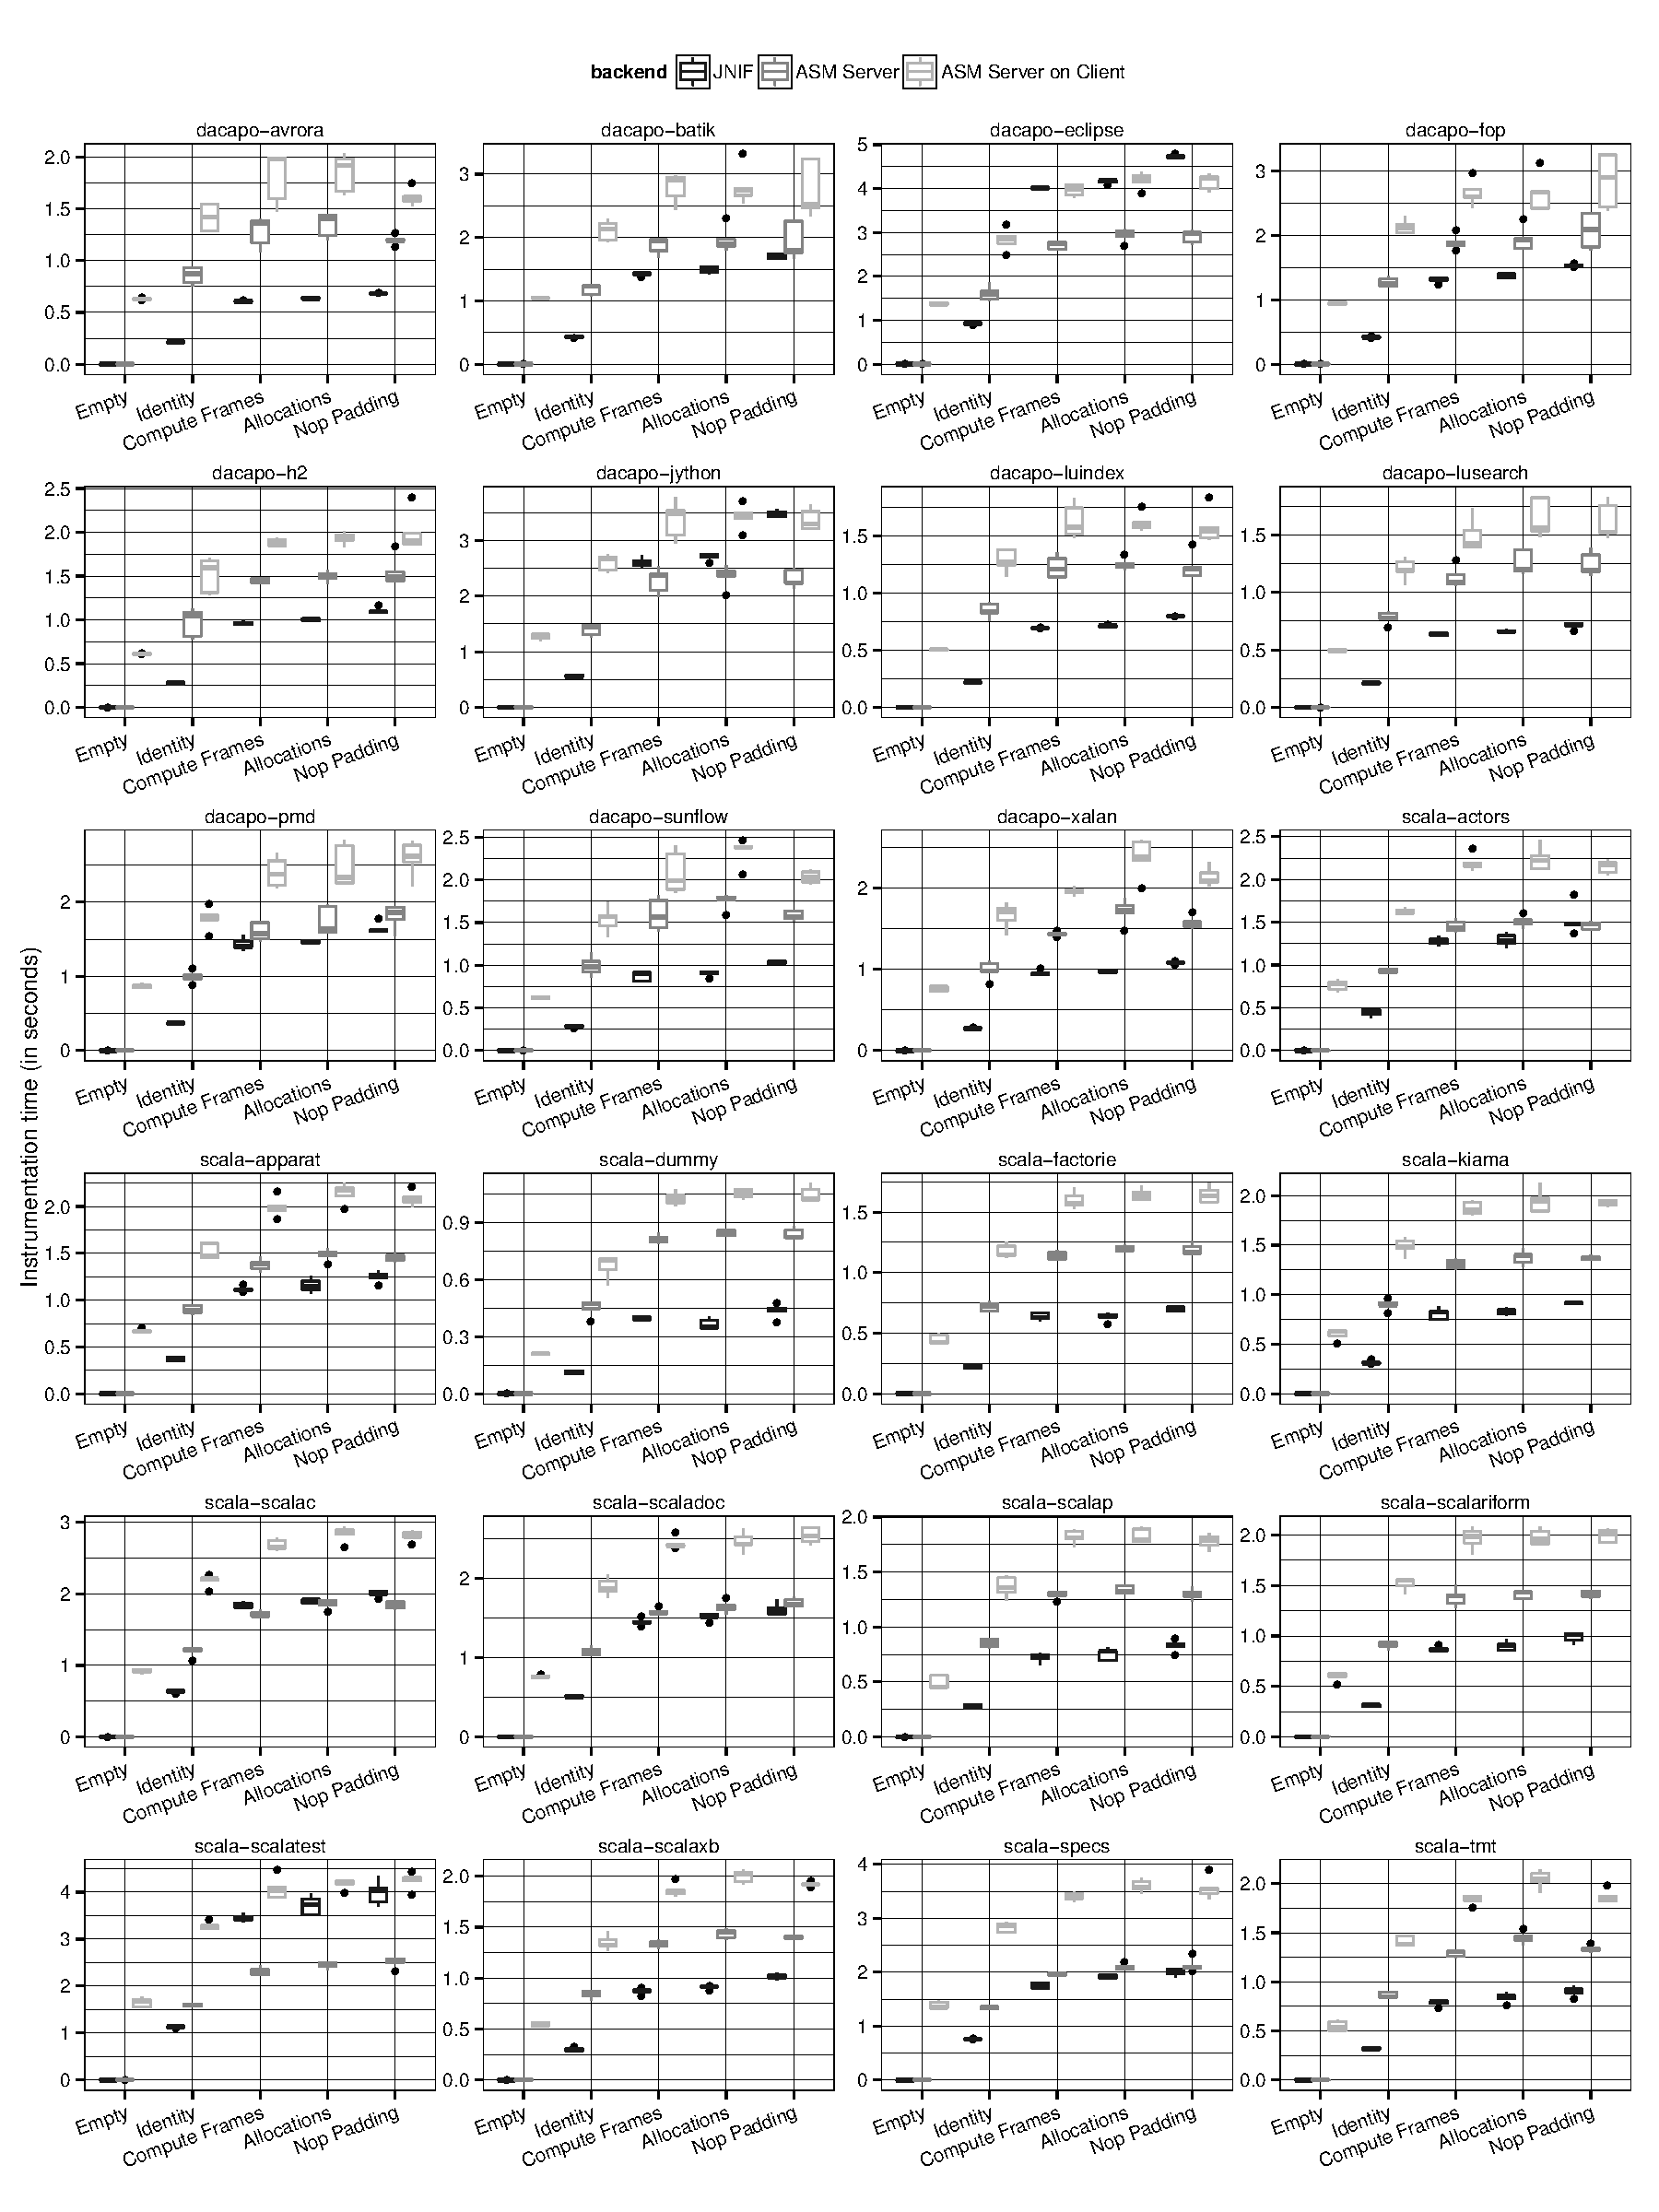
\includegraphics[width=\textwidth]{chapters/jnif/eval-all-chart-instr}

\vspace{-5mm}
\caption{Instrumentation time on DaCapo and Scala benchmarks}
\label{fig:instr-time}
\end{figure*}

%\chart{eval-dacapo-chart-instr}{Instrumentation time on DaCapo}{fig:instr-time-dacapo}
%\chart{eval-scala-chart-instr}{Instrumentation time on Scala and JRuby}{fig:instr-time-scala}

\subsection*{Reproducibility}

To run these evaluations, a Makefile script is provided in the git repository.
These tasks take care of the compilation of the JNIF library and also all java files needed. 
The repository is self-contained, no need to download dacapo benchmarks separately.

\begin{lstlisting}[caption=Running testapp,label=usage-parse2]
> make testapp
\end{lstlisting}

\begin{lstlisting}[caption=Running dacapo,label=usage-parse3]
> make testapp
\end{lstlisting}

To run a particular dacapo benchmark with default settings

\begin{lstlisting}[caption=Running dacapo,label=usage-parse4]
> make dacapo BENCH=avrora
\end{lstlisting}

To run a full evaluation with all dacapo benchmarks in all configuration a task -eval- is provided. You can set how many times run each configuration with the variable times, like

\begin{lstlisting}[caption=Running full eval five times,label=usage-parse5]
> make eval times=5
\end{lstlisting}

Finally, there is a task to create plots for the evaluation. This task needs R with the package ggplot2.

\begin{lstlisting}[caption=Plots,label=usage-parse6]
> make plots
\end{lstlisting}

%1. Stand-alone test-unit:
%In this stage we only test basic functionality of the API such as get the
%right size and the ability to parse and write without correctly without
%any modification and with them. The use of this kind of tests rely on the
%property of the API that if no modification is done to the model the 
%writer is able to recover the original bytes of the class files (except with
%the non-unique property of the stack map tables).
%
%2. Minimal native agent:
%At this stage we prepared several kind of transformations (instrumentation)
%including the identity transformation to test if model/parser/analysis/writer
%can be executed correctly inside a JVM.
%
%3. Dacapo benchmarks:
%As the final tests we run those instrumentations on the Dacapo benchmarks 
%to stress the API. Moreover we use this stage to perform our evaluation.
